\begin{figure}[h]
    \centering
    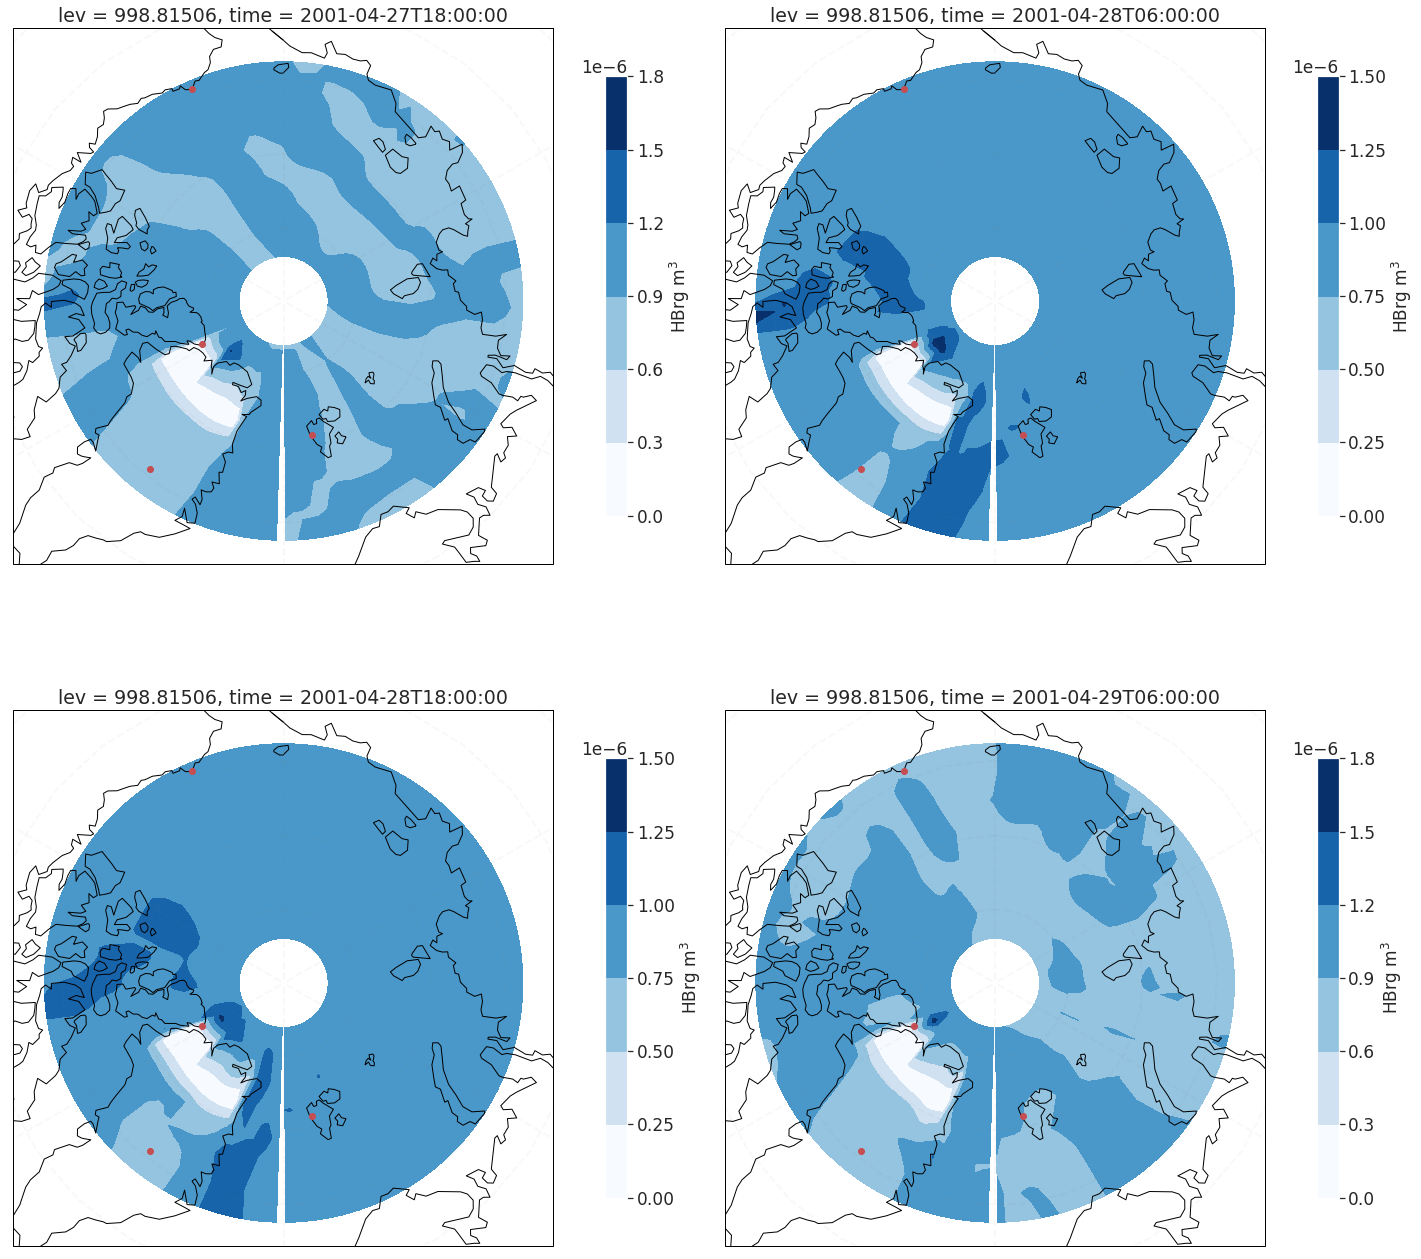
\includegraphics[width=\linewidth]{Chapter6_Results/images/polarHBr_HTWO_step3.png}
    \caption{Concentration ($g m^{-3}$) of \chem{HBr} in the first model layer the Arctic at 18:00 and 06:00 (UTC) of the 27th, 28th and 29th of April, 2001. The result is from the test including hard-coded photodissociation rates as well as a new (high) Henry-coefficient at HTWO resolution. The red dots are the positions of the stations with observations in 2001 (see the map in Figure \ref{fig:stns} for reference)}
    \label{fig:polarHBr_HTWO_step3}
\end{figure}